\documentclass[conference]{IEEEtran}
\usepackage{graphicx}
\begin{document}
\title{Word Hunter}
\author{\IEEEauthorblockN{Yang Zhao}
\IEEEauthorblockA{yzhao3@stanford.edu}
\and
\IEEEauthorblockN{Shuo Liu}
\IEEEauthorblockA{shuol@stanford.edu}
\and
\IEEEauthorblockN{Lingren Zhang}
\IEEEauthorblockA{lz7@stanford.edu}
}

% make the title area
\maketitle


\begin{abstract}
For this project we propose and implement a reading tool on Andriod platform that can be used to identify keywords on paper-based media.  After receiving an image of the media, we first pre-process the image (binarization and de-skew), and then use OCR (in particular, Tesseract OCR engine) to recognize the text and find the keywords, at last we highlight the keywords by circling it with a red box.
\end{abstract}

\section{Introduction}
Have you ever read a long paper-based article and find yourself unable to locate keywords? With the advancement of digital media, sometimes we take basic word search for granted. But the world is still full of media printed on paper and it would make our lives much simpler if we can automate this basic reading tool for good old fashioned books. We propose a mobile application that will be able to find a word that the user specified through a phone’s viewfinder. As soon as the phone detects the word it will highlight it, saving the user many minutes of looking for the word him/herself. 

For example, we want to search for “nonlinear equation” in this page of paper. We only need to use our smart phone to scan over the paper. Whenever the word “nonlinear equation” appears on the phone screen, it will be immediately circled in red.\\

\begin{figure}
\center
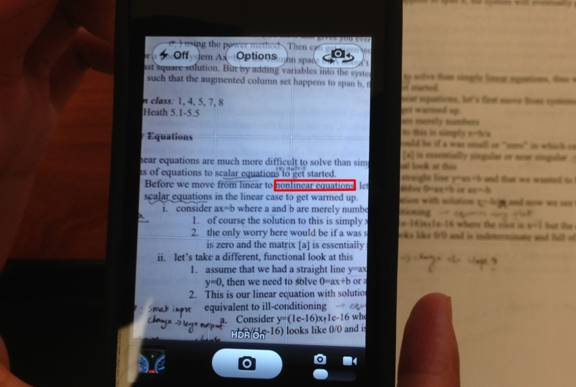
\includegraphics[scale=0.5]{demo.jpg}
\caption{Word Hunter Demo}
\end{figure}

\section{Preprocessing}
include sample image (original)
\subsection{Binarization}

First step is to enhance the image by histogram equalization, which can be done by calling OpenCV function equalizeHist.  The idea is to achieve uniform distribution of gray level in the image, without changing the relative brightness of the image. (i.e. if pixel A is brighter than pixel B in the original image, A will still be brighter than B in the histogram-equalized image)

The second step is to use an adaptive thresholding algorithm to separate text from background.  The reason we choose adaptive thresholding instead of global thresholding is that the lighting/brightness of the image is not uniform which will cause global thresholding to perform poorly in the extreme bright/dark regions.  We also observed that blocksize=25 yields the best thresholding result.

include sample image after binarization

\subsection{De-skew}

include sample image after de-skew.

\subsection{Layout analysis}

\section{Word Recognition}

\section{Conclusion}

\section*{Acknowledgment}
We would like to thank David Chen and Sam Tsai for their generous and responsive help on the project.


%\begin{thebibliography}{1}
%\bibitem{IEEEhowto:kopka}
%H.~Kopka and P.~W. Daly, \emph{A Guide to \LaTeX}, 3rd~ed.\hskip 1em plus
%  0.5em minus 0.4em\relax Harlow, England: Addison-Wesley, 1999.
%\end{thebibliography}

\end{document}